\documentclass[10pt, hyperref={pdfpagelabels=false}]{beamer}

\usepackage{tikz, verbatim, enumitem}

\usetikzlibrary{decorations}
\usetikzlibrary{backgrounds}
\usetikzlibrary{patterns}
\usetikzlibrary{snakes}
\usetikzlibrary{shapes}
\usetikzlibrary{positioning, shapes.geometric, arrows.meta}
\usetikzlibrary{arrows,automata}

\setlength{\parindent}{0pt}
\setlength{\parskip}{1.3ex}

\title{The TCP Protocol Stack}
\author{Michael Brockway}
\date{\today}

\setlist[enumerate]{itemsep=0mm}
\setitemize{label=\usebeamerfont*{itemize item}
  \usebeamercolor[fg]{itemize item}
  \usebeamertemplate{itemize item}}

\begin{document}

\begin{frame}
\titlepage
\end{frame}

\begin{frame}
\frametitle{Introduction - Layered archtecture}
Networking software is desgined in a layered fashion
\begin{itemize}
\item The bottom layer is the services offered by the underlying hardware and their device drivers: 'Ethernet', 'Wifi', 'BlueTooth', 'Zigbee' all employ electronics to get digital signals from one computing \emph{host} to another.
\item The next layer is software that employs the lower layer functionality to  provide a higher (more abstract) level of service.
\item There will be a sequence of layers each employing the services of the layer below.
\end{itemize}
\end{frame}

\begin{frame}
\frametitle{Example}
\begin{center}
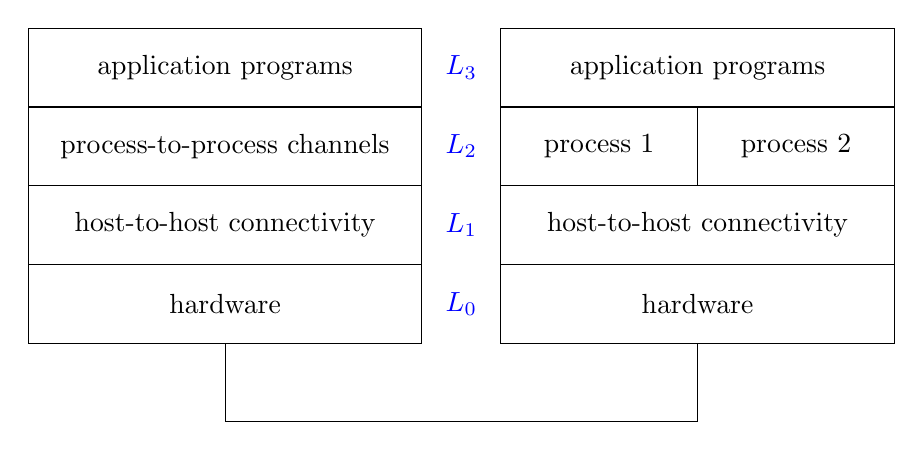
\begin{tikzpicture} [minimum height=1, draw]
  \draw (0,6) rectangle (5,7); \draw (2.5,6.5) node {application programs}; 
  \draw (0,5) rectangle (5,6); \draw (2.5,5.5) node {process-to-process channels}; 
  \draw (0,4) rectangle (5,5); \draw (2.5,4.5) node {host-to-host connectivity}; 
  \draw (0,3) rectangle (5,4); \draw (2.5,3.5) node {hardware}; 

  \draw (6,6) rectangle (11,7); \draw (8.5,6.5) node {application programs}; 
  \draw (6,5) rectangle (11,6); \draw (8.5,5)--(8.5,6);
  \draw (7.25,5.5) node {process 1}; \draw (9.75,5.5) node {process 2}; 
  \draw (6,4) rectangle (11,5); \draw (8.5,4.5) node {host-to-host connectivity}; 
  \draw (6,3) rectangle (11,4); \draw (8.5,3.5) node {hardware}; 

  \draw (5.5,3.5) node[color=blue] {$L_0$}; \draw (5.5,4.5) node[color=blue] {$L_1$};   
  \draw (5.5,5.5) node[color=blue] {$L_2$}; \draw (5.5,6.5) node[color=blue] {$L_3$};   

  \draw (2.5,3) -- (2.5,2) -- (8.5,2) -- (8.5,3);
\end{tikzpicture}
\begin{itemize}
\item The host-to-host connectivity software employs the hardware and its device-drivers to send data to another host.
\item The software driving a process uses this to exchange data with a peer process on another host.
\item Application software uses process-to-process service software to exchange data with another app on another host.
\end{itemize} 
\end{center}
\end{frame}

\begin{frame}
\frametitle{Layered architecture}
Each layer implements one (or more) protocol. 

Each protocol defines
\begin{itemize}
\item a \emph{\color{blue}service interface}: in later $L_i$, defines operations provided by this protocol for layer $L_{i+1}$
\item a \emph{\color{blue}peer-to-peer interface}: defines the messages exchanged with a \emph{peer} in layer  $L_i$.
\item At the hardware level $L_0$ peer-to-peer communication is directly over a link;
\item at a higher level $L_i$, $L_i$ to $L_i$ communication is \emph{conceptual}; in reality it happens by $L_i$ making use of services of $L_{i-1}$ which uses services of $L_{i-2}$ and so on down to $L_0$.
\end{itemize}
\end{frame}

\begin{frame}
\frametitle{Example}
A application program sending data to a peer using request-reply protocol over host-to-host protocol.

\begin{center}
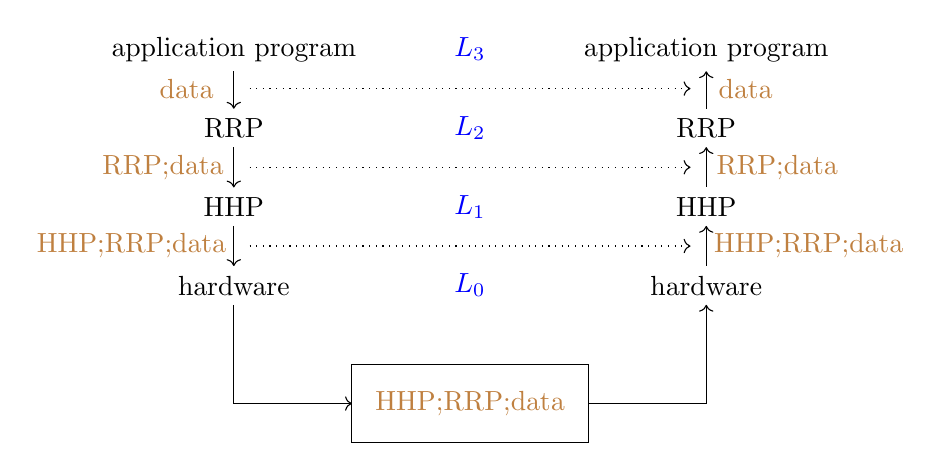
\begin{tikzpicture} [minimum height=1, draw]
  \draw (2.5,6.5) node (app1) {application program}; 
  \draw (2.5,5.5) node (rrp1) {RRP}; 
  \draw (2.5,4.5) node (hhp1) {HHP}; 
  \draw (2.5,3.5) node (hrd1) {hardware}; 

  \draw (8.5,6.5) node (app2) {application program}; 
  \draw (8.5,5.5) node (rrp2) {RRP}; 
  \draw (8.5,4.5) node (hhp2) {HHP}; 
  \draw (8.5,3.5) node (hrd2) {hardware}; 

  \draw (5.5,3.5) node[color=blue] {$L_0$}; \draw (5.5,4.5) node[color=blue] {$L_1$};   
  \draw (5.5,5.5) node[color=blue] {$L_2$}; \draw (5.5,6.5) node[color=blue] {$L_3$};   

  \path (app1) edge[->] (rrp1)
        (rrp1) edge[->] (hhp1)
        (hhp1) edge[->] (hrd1);
  \path (app2) edge[<-] (rrp2)
        (rrp2) edge[<-] (hhp2)
        (hhp2) edge[<-] (hrd2);

  \draw (1.9,6) node[color=brown] {data};
  \draw (1.6,5) node[color=brown] {RRP;data};
  \draw (1.2,4) node[color=brown] {HHP;RRP;data};
  \draw (5.5,2) node[color=brown] (m) {HHP;RRP;data};
   \draw (9,6) node[color=brown] {data};
  \draw (9.4,5) node[color=brown] {RRP;data};
  \draw (9.8,4) node[color=brown] {HHP;RRP;data};
  
  \draw [->] (hrd1) -- (2.5,2) -- (4,2);
  \draw (4,1.5) rectangle (7,2.5);
  \draw [->] (7,2) -- (8.5,2) -- (hrd2);
  \draw [->, dotted] (2.7,6) -- (8.3,6);
  \draw [->, dotted] (2.7,5) -- (8.3,5);
  \draw [->, dotted] (2.7,4) -- (8.3,4);
\end{tikzpicture}
\end{center}
\end{frame}

\begin{frame}
\frametitle{Example}
The application on host 1 sends a message to an application on host2. In practice this the application calls a
function in service interface of the Request Reply Protocol software module.

The dotted lines show \emph{virtual} communication between peer entities.
\begin{itemize}
\item RRP attaches some control information in an \emph{RRP header} to data so that its peer RRP will know what to do when the data is received by it. This combined message is sent to the local host-to-host protocol.
\item HHP attaches HHP-specific header, and
\item the entire message is sent to host 2
\end{itemize}

Each layer attaches a header (encapsulates the message) as the message ‘goes down’.

At host 2, each layer removes its header, performs header specific
processing and passes the message ‘up’.
\end{frame}

\begin{frame}
\frametitle{The ISO seven layer \emph{open systems interconnection} model}
\begin{itemize}
\item[$L_1$] Physical Layer: network hardware; mechanical and electrical connections.
\item[$L_2$] Data Link Layer: managed the transmission of data across the physical network. Framing, data transparency and error control.
\item[$L_3$] Network Layer: define how addresses are assigned and how data is forwarded from one network to another: routing
\item[$L_4$] Transport Layer: Provides reliable, transparent transfer of data between end points. End to end Error recovery and flow control
\item[$L_5$] Session Layer: Provides the control structure for communication between applications. Establishes, manages and terminates dialogues between application entities. Specifies security details.
\item[$L_6$] Presentation Layer: Provides independence to the application process from differences in data representation.
\item[$L_7$] Application Layer: Each protocol specifies how a particular application uses the network and how an application program on one computer makes a request and how the application on another machine responds.
\end{itemize}
\end{frame}

\begin{frame}
\frametitle{ISO/OSI and TCP/IP}
The seven-layer model had this many layers to provide for compatibility between network teachnologies. 

In practice TCP is \emph{the} standard network technology and protocol suit of the internet. It manages with four layers which correspond to the seven-layer model as follows -
\begin{center}
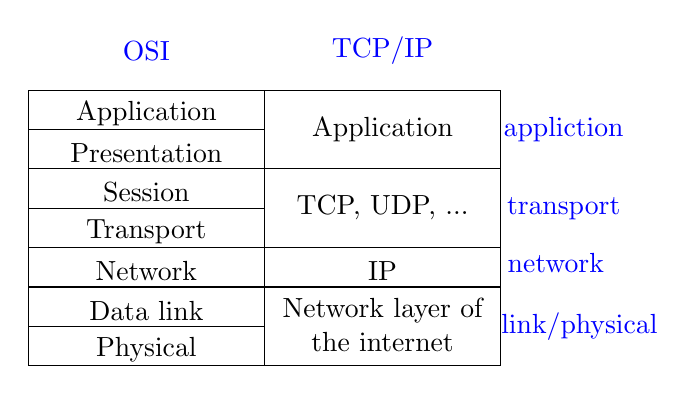
\begin{tikzpicture} [minimum height=1, draw]
  \draw (1.5, 7) node[color=blue] {OSI}; \draw (4.5, 7) node[color=blue] {TCP/IP};
  \draw (0,6.0) rectangle (3,6.5); \draw (1.5,6.2) node {Application}; 
  \draw (0,5.5) rectangle (3,6.0); \draw (1.5,5.7) node {Presentation};
  \draw (0,5.0) rectangle (3,5.5); \draw (1.5,5.2) node {Session}; 
  \draw (0,4.5) rectangle (3,5.0); \draw (1.5,4.7) node {Transport}; 
  \draw (0,4.0) rectangle (3,4.5); \draw (1.5,4.2) node {Network}; 
  \draw (0,3.5) rectangle (3,4.0); \draw (1.5,3.7) node {Data link}; 
  \draw (0,3.0) rectangle (3,3.5); \draw (1.5,3.2) node {Physical}; 

  \draw (3,5.5) rectangle (6,6.5); \draw (4.5,6.0) node {Application}; 
  \draw (3,4.5) rectangle (6,5.5); \draw (4.5,5.0) node {TCP, UDP, ...}; 
  \draw (3,4.0) rectangle (6,4.5); \draw (4.5,4.2) node {IP}; 
  \draw (3,3.0) rectangle (6,4.0); \draw (4.5,3.7) node {Network layer of}; 
                                   \draw (4.5,3.3) node {the internet}; 

  \draw (6.8,6.0) node[color=blue] {appliction};
  \draw (6.8,5.0) node[color=blue] {transport};
  \draw (6.7,4.3) node[color=blue] {network};
  \draw (7.0,3.5) node[color=blue] {link/physical};

\end{tikzpicture}
\end{center}
\end{frame}

\begin{frame}
\frametitle{TCP/IP}
\begin{itemize}
\item TCP/IP (Transmission Control Protocol / Internet Protocol) is the internet’s communications standard
\item It is a complete suite of protocols and includes network, transport and application layers.
\item It is used in many Unix systems, began in the Unix world; Unix is used widely throughout the Internet.
\end{itemize}

TCP/IP applications (application-layer protocols) include
\begin{itemize}
\item[FTP] file transfer protocol: nowadays wrapped in a security layer; eg Filezilla
\item[Telnet] for remote log-in to a server. Now in a security later; eg SSH
\item[DHS] Domain Name Service.
\item[SNMP] Simple Network Management Protocol.
\item[SNTP] Simple Mail Transfer Protocol.
\item[HTTP] Hypertext transfer protocol - used by web browsers.
\end{itemize}
\end{frame}

\begin{frame}
\frametitle{TCP (Transport layer)}
\begin{itemize}
\item \emph{\color{blue}Transmission Control Protocol}.
\item Reliable: TCP service takes responsibility for correct delivery of the data to peer; arranges for re-send if a data packet is lost or corrupt;
\item \emph{\color{blue}connection-oriented} (see below);
\item fragments an incoming byte stream into messages for IP layer;
\item reassembles received messages (passed up from IP layer) in correct order, to create an output stream;
\item manages flow control.
\end{itemize}

Connection-oriented
\begin{itemize}
\item Communication starts by establising a connection or \emph{\color{blue}virtual circuit} to peer;
\item Data sent either way between peers all follows the same route: goes via the connection;
\item Connection is closed (virtual circuit destroyed) at end of `conversation'.
\item This software construct is how TCP manages reliable tranport of data in correct order and without data duplication or loss.
\end{itemize}
\end{frame}

\begin{frame}
\frametitle{UDP (Transport layer)}
\begin{itemize}
\item \emph{\color{blue}User Datagram Protocol}.
\item A `best effort' service: data errors are detected but no responsibility re-sending. The application has to handle lost or corrupt data.
\item \emph{\color{blue}connectionless}; Data transimissions - \emph{\color{blue}UDP datagrams} are separate from one another; each is individually addressed to recipient.
\item no sequencing or flow-control.
\end{itemize}

TCP or UDP?
\begin{itemize}
\item UDP is light-weight compared with TCP; it has much less work to do compared with TCP.
\item Preferred in applications which require many short messages to be sent at high speed: VOIP (telephony), audio, video streaming, ...
\item TCP preferred where data exchanges are more `heavy-weight': HTTP, WWW
\end{itemize}
\end{frame}

\begin{frame}
\frametitle{Transport layer data}
\begin{figure}[!htb]
\begin{center}
\includegraphics[width=01.2\textwidth]{TCPUDPSegs.pdf}
\end{center}
\end{figure}
\end{frame}

\begin{frame}
\frametitle{Transport layer data}
Port numbers define the ends of logical connections.
\begin{itemize}
\item a message from a process on a host will go to a process on the destination host using the appropriate port number.
\end{itemize}
\end{frame}

\begin{frame}
\frametitle{IP layer}
IP
\begin{itemize}
\item \emph{\color{blue}Internet Protocol}:
\item an `unreliable' connectionless best effort IP packet delivery service.
\item A question for you to think about: the IP service interface supports both \emph{reliable} TCP and emph{best-effort} UDP. How does an `unreliable' or best-effort-only service sipport a \emph{reliable} service?
\item Addressing
\item Routing
\end{itemize}

ARP / RARP
\begin{itemize}
\item (Reverse) Address Resolution Protocol
\item Maps IP addresses onto data link layer addresses such as Ethernet card addresses: eg 193.63.32.233 to (MAC address) 008002B39DD10
\item Its functions are defined as part of TCP/IP but its implementation is dependent on the network type.
\item TCP/IP does not define what happens below the IP layer.
\end{itemize}
\end{frame}

\begin{frame}
\frametitle{Transport layer data}
\begin{figure}[!htb]
\begin{center}
\includegraphics[width=1.2\textwidth]{IPDatagramFmt.pdf}
\end{center}
\end{figure}
\end{frame}

\begin{frame}
\frametitle{32-bit IP Addresses}
32 bit addresses specify sources and target hosts.
\begin{itemize}
\item normally represented in \emph{dotted decimal format}, each block describing 8 bits: thus 193.63.32.233 is the sames as 0xC13F20E9 or in binary, 11000001 00111111 00100000 11101001
\item Each IP address has two components: the higher bits identify a local network; the lower bits an individual host or interface to a router, within a network.
\item Hosts on the same network must have IP addresses with the same network part, but different host parts.
\item Hosts with different network address parts might be connected by a router (eg, with two interfaces with network parts agreeing with the two hosts).
\item Originally the network part was 8, 16, or 24 bits (class A, B or C); now using CIDR (classless interdomain routing) and VLSM (variable-length subnet masking) can be any size.
  \begin{itemize}
  \item eg 223.1.252.3 within the subnet 223.1.252.0/22 would need subnet mask 255.255.252.0, in binary, 11111111 11111111 11111100 00000000: 22 bits' network part.
  \end{itemize}
\end{itemize}
\end{frame}

\begin{frame}
\frametitle{Domain names}
To avoid referring to individual numerical IP addresses the concepts of \emph{domain names} and \emph{host names} developed.
\begin{itemize}
\item Domain and host names are mapped to IP addresses.
\item cougar.unn.ac.uk $\longrightarrow$ 193.63.32.233;
\item \emph{no} logical relationship between the parts of an IP address and its domain name.
\item The mapping is done using \emph{Domain Name Resolution}, normally with the help of a \emph{Domain Name Server}.
\end{itemize}

There are not enough 32-bit addresses!
\begin{itemize}
\item More than $2^{32}$ (4 billion) addresses are needed.
\item For many years the internet has 'coped' by allowing addresses to be duplicated, with routers doing IP address `translation' to prevent address clashes outside of LANs.
\item this makes DNS especially handy!
\item IP v 6 specifies 64-bit addresses -  clean resoltution of the problem but IP v 6 is very slow to be adopted by users.
\end{itemize}
\end{frame}

\begin{frame}
\frametitle{Programming TCP connection}
The focus is on applications using transport layer services, especially TCP, UDP; useful for development of \emph{distributed} applications. The basic software entity is a \emph{\color{blue}socket}.
\begin{itemize}
\item role similar to a file-handle;
\item First, the socket is connected to a remote host (compare with opening a file); then data is input/output through the socket; when complete, the socket is closed – the connection is broken.
\item Implemented in Java using package \texttt{java.net}, espectially class \texttt{java.net.Socket}.
\item C provides the socket class and a library of socket functions prototyped in \texttt{<sys/socket.h>}.
\end{itemize}
\end{frame}

\begin{frame}
\frametitle{Programming TCP connections}
\texttt{\#include <sys/socket.h>}
\begin{itemize}
\item \texttt{\color{blue}int socket(...)}; creates a new socket
\item \texttt{\color{blue} int gethostname(char *name, int namelen)}; translates a host name to an ip address
\item \texttt{\color{blue} int bind(int s, struct sockaddr *name, int namelen)}; binds a socket to a specific address (and port)
\item \texttt{\color{blue} int connect(int s, struct sockaddr *addr, int *addrlen)}; used by client to request a socket connection to a remote address (and port)
\item \texttt{\color{blue}void listen (socket\_id s, int backlog )}; causes server to start listening for requests for a connection
\item \texttt{\color{blue}int accept(int s, struct sockaddr *addr, int *addrlen)}; used by server to accept a connection request from a client
\item \texttt{\color{blue}int read(int d, char *buf, int nbytes)};
\item \texttt{\color{blue}int write(int d, char *buf, int nb)}; d = socket id; reads from/writes to a socket
\item \texttt{\color{blue}int close(int d)};
\end{itemize}
\end{frame}

\begin{frame} [fragile]
\frametitle{TCP server logic}
In general, the behaviour you have to program is dependent on the state of the system. There you tend to write such constructs as
{\color{blue}
\begin{verbatim}
Fix the port number
Create a socket for the server
Start listening on the socket for requests to connect
Repeat –
  Wait for a request for a connection.
  Accept function returns id of a new socket which will manage the
    connection; also gets the name of the client host.
  Spin off a new thread to serve the client;
\end{verbatim}
}

Serving the client
\begin{itemize}
\item A subroutine running in a new thread
\item Uses socket returned by Accept function
\item Uses socket I/O functions to send data to / receive data from client according to protocol
\item When finished, closes the socket.
\end{itemize}
\end{frame}

\begin{frame} [fragile]
\frametitle{TCP client logic}
In general, the behaviour you have to program is dependent on the state of the system. There you tend to write such constructs as
{\color{blue}
\begin{verbatim}
Specify server name/addr, port num to which we wish to connect;
Create a socket;
Bind this socket to host name and port number;
Request a connection to the server host / port;
if (return value indicates connection successful)
 use socket I/O functions to send data to/receive data;
Close the socket when finished.
\end{verbatim}
}
\begin{itemize}
\item The port number is same at both ends: 
  identifies the virtual circuit between the client and server.
\end{itemize}
\end{frame}

\begin{frame} [fragile]
\frametitle{Programming UDP}
Again use a \emph{\color{blue}socket} but no connection is established. Instead,
a version of the send function is used which incorporates a destination address parameter:
{\color{blue}
\begin{verbatim}
int sendto(int sockID, char * msg,
   unsigned int msgLen, int flags,
   struct sockaddr * destAddress,
   unsigned int addressLen)
\end{verbatim}
}

...and a version of the receive function is used which incorporates a source address
parameter:
{\color{blue}
\begin{verbatim}
int recvfrom(int sockID, char * msg,
   unsigned int msgLen, int flags,
   struct sockaddr * sourceAddress,
   unsigned int * addressLen)
\end{verbatim}
}

The return value in each case is the number of bytes sent/received. Note is the use of pointers to provide in/out parameters: note the int * (rather than int) for the receive function's address length parameter.
\end{frame}

\begin{frame}
\frametitle{Further reading}
RFC1122 Requirements for Internet Hosts – Communication Layers
\begin{itemize}
\item \texttt{https://en.wikipedia.org/wiki/Internet\_protocol\_suite}
\item \texttt{https://www.w3.org/People/Frystyk/thesis/TcpIp.html}
\item \texttt{\small https://en.wikibooks.org/wiki/A-level\_Computing/AQA/\\Computer\_Components,\_The\_Stored\_Program\_Concept\_and\_the\_Internet/\\Structure\_of\_the\_Internet}
\end{itemize}

Requests for comment (RFCs): the following are easily found by internet search:
\begin{itemize}
\item RFC1123 Requirements for Internet Hosts – Application and Support
\item RFC768 User Datagram Protocol
\item RFC793 TRANSMISSION CONTROL PROTOCOL
\end{itemize}


\end{frame}

\end{document}

